\documentclass[psamsfonts]{amsart}

%-------Packages---------
\usepackage{amssymb,amsfonts}
\usepackage{semantic}
\usepackage{fullpage}
\usepackage{tikz-cd}
\usepackage{todonotes}
\usepackage{physics}
\usepackage[all,arc]{xy}
\usepackage{enumerate}
\usepackage{enumitem}
\usepackage{mathrsfs}
\usepackage{theoremref}
\usepackage{graphicx}
\usepackage[bookmarks]{hyperref}

%--------Theorem Environments--------
%theoremstyle{plain} --- default
\newtheorem{thm}{Theorem}[section]
\newtheorem{cor}[thm]{Corollary}
\newtheorem{prop}[thm]{Proposition}
\newtheorem{lem}[thm]{Lemma}
\newtheorem{conj}[thm]{Conjecture}
\newtheorem{quest}[thm]{Question}

\theoremstyle{definition}
\newtheorem{defn}[thm]{Definition}
\newtheorem{defns}[thm]{Definitions}
\newtheorem{con}[thm]{Construction}
\newtheorem{exmp}[thm]{Example}
\newtheorem{exmps}[thm]{Examples}
\newtheorem{notn}[thm]{Notation}
\newtheorem{notns}[thm]{Notations}
\newtheorem{addm}[thm]{Addendum}
\newtheorem{exer}[thm]{Exercise}
\newtheorem{innercustomexer}{Exercise}
\newenvironment{customexer}[1]
  {\renewcommand\theinnercustomexer{#1}\innercustomexer}
  {\endinnercustomexer}

\newtheorem{innercustomprob}{Problem}
\newenvironment{customprob}[1]
  {\renewcommand\theinnercustomprob{#1}\innercustomprob}
  {\endinnercustomprob}

\newtheorem{innercustomthm}{Proposition}
\newenvironment{customthm}[1]
  {\renewcommand\theinnercustomthm{#1}\innercustomthm}
  {\endinnercustomthm}

\newtheorem{innercustomexmp}{Example}
\newenvironment{customexmp}[1]
  {\renewcommand\theinnercustomthm{#1}\innercustomthm}
  {\endinnercustomthm}

\theoremstyle{remar}
\newtheorem*{rem}{Remark}
\newtheorem{rems}[thm]{Remarks}
\newtheorem{warn}[thm]{Warning}
\newtheorem{sch}[thm]{Scholium}

\DeclareMathOperator{\Hom}{Hom}
\DeclareMathOperator{\Id}{Id}
\DeclareMathOperator{\End}{End}
\DeclareMathOperator{\ord}{ord}
\DeclareMathOperator{\Aut}{Aut}
\DeclareMathOperator{\Gal}{Gal}
\DeclareMathOperator{\RP}{\mathbb{R}\mathbb{P}}
\DeclareMathOperator{\Int}{Int}
\DeclareMathOperator{\bd}{bd}
\DeclareMathOperator{\supp}{supp}

\makeatletter
\let\c@equation\c@thm
\makeatother
\numberwithin{equation}{section}

\bibliographystyle{plain}

\begin{document}

\title{Introduction to Smooth Manifolds}
\author{Hidenori Shinohara}

\maketitle
\tableofcontents

\section{Chapter 1: Smooth Manifolds}
\subsection{Exercises}
\begin{customexer}{1.1}\label{exercise_1_1}
  Show that equivalent definitions of manifolds are obtained if instead of allowing $U$ to be homeomorphic to \textit{any} open subset of $\mathbb{R}^n$, we require it to be homeomorphic to an open ball in $\mathbb{R}^n$, or to $\mathbb{R}^n$ itself.
\end{customexer}

\begin{proof}
  It is clear that a ``manifold" satisfying the open-ball or $\mathbb{R}^n$ definition satisfies the open-subset definition.
  Let $M$ be a manifold satisfying the open-subset definition.
  Let $x \in M$ be given and let $U, \hat{U}, \phi$ be given according to the definition.
  Since $\hat{U}$ is open, there exists an open ball $B$ such that $\phi(x) \in B \subset \hat{U}$.
  Restrict $\phi$ to $\phi^{-1}(B)$.
  Then $\phi^{-1}(B)$ is an open subset of $M$ containing $x$, and $\phi\mid_{\phi^{-1}(B)}$ is a homeomorphism between $\phi^{-1}(B)$ and $B$.
  Thus $M$ satisfies the open-ball definition.

  $B(x, r) \subset \mathbb{R}^n$ is homeomorphic to $\mathbb{R}^n$ by the map $(x_1 + a_1, \cdots, x_n + a_n) \mapsto (\frac{a_1}{r - a_1}, \cdots, \frac{a_n}{r - a_n})$ where $x = (x_1, \cdots, x_n)$ is the center of $B(x, r)$ and $r$ is the radius.
  Since the composition of two homeomorphisms gives a homeomorphism, $M$ also satisfies the $\mathbb{R}^n$ definition as well.
\end{proof}


\begin{customexer}{1.6}
  Show that $\RP^n$ is Hausdorff and second-countable, and is therefore a topological $n$-manifold.
\end{customexer}

\begin{proof}
  From the definition of $\pi$, it is easy to see that $\pi(B(x, r))$ is open in $\RP^n$ where $x \in S^n$ and $0 < r < 1$.

  Let $[x], [y] \in \RP^n$ be given.
  Without loss of generality, assume $x, y \in S^{n}$.
  Let $r = \min\{ \abs{x - y}, \abs{x + y}, 1 \} / 2$.
  Then $U_x = \pi(B(x, r)), U_y = \pi(B(y, r))$ contain $[x], [y]$, respectively.
  $\pi^{-1}(U_x), \pi^{-1}(U_y)$ are both open in $\mathbb{R}^{n + 1} \setminus \{ 0 \}$ which can be seen easily by writing down exactly which points belong to them, so $U_x, U_y$ are both open in $\RP^n$.
  Then $\pi^{-1}(U_x \cap U_y) = \pi^{-1}(U_x) \cap \pi^{-1}(U_y) = \emptyset$, so $U_x \cap U_y = \emptyset$.
  Therefore, $\RP^n$ is Hausdorff.

  Let $\mathcal{B} = \{ \pi(B(x, 1 / k)) \mid x \in \mathbb{Q}^{n + 1} \cap S^{n}, k \in \{ 2, 3, 4, \cdots \} \}$.
  Then $\mathcal{B}$ is a countable collection of open sets whose union is $\RP^n$.
  Let $U \subset \RP^n$ be a nonempty open set.
  Let $[x] \in U$.
  Since $\pi$ is a quotient map, $\pi^{-1}(U)$ is open.
  Moreover, $x \in \pi^{-1}(U)$.
  Without loss of generality, $x \in S^{n}$.
  Then $x \in B(x', 1 / k) \subset \pi^{-1}(U)$ for some $B(x', 1 / k) \in \mathcal{B}$.
  Then $[x] = \pi(x) \in \pi(B(x', 1 / k)) \subset \pi(\pi^{-1}(U)) = U$.
  Therefore, $\mathcal{B}$ is a countable basis of $\RP^n$.
\end{proof}

\begin{customexer}{1.7}
  Show that $\RP^n$ is compact.
\end{customexer}

\begin{proof}
  $\pi(S^n) = \RP^n$ and $S^n$ is compact because it is a closed, bounded subset of $\mathbb{R}^{n + 1}$. (Heine-Borel)
  Moreover, the image of a compact set under a continuous map is compact. (See A.45(a))
  Thus $\RP^n$ is compact.
\end{proof}

\begin{customexer}{1.14}
  Suppose $\mathcal{X}$ is a locally finite collection of subsets of a topological space $M$.
  \begin{enumerate}[label=(\alph*)]
    \item 
      The collection $\{ \overline{X} : X \in \mathcal{X} \}$ is also locally finite.
    \item
      $\overline{\bigcup_{X \in \mathcal{X}} X} = \bigcup_{X \in \mathcal{X}} \overline{X}$.
  \end{enumerate}
\end{customexer}

\begin{proof}
  $ $
  \begin{enumerate}[label=(\alph*)]
    \item
      Let $p \in M$.
      Then there exists an open set $U$ containing $x$ such that there are only finitely many $X \in \mathcal{X}$ such that $U \cap X \ne \emptyset$.
      Let $X \in \mathcal{X}$.
      \begin{itemize}
        \item
          If $U \cap X \ne \emptyset$, then $U \cap \overline{X} \supset U \cap X \ne \emptyset$.
        \item
          If $U \cap X = \emptyset$, then $U^c$ is closed, so $\overline{X} \subset U^c$.
          In other words, $U \cap \overline{X} = \emptyset$.
      \end{itemize}
      This shows that the number of $X \in \mathcal{X}$ that intersects $U$ and the number of $\overline{X} \in \mathcal{X}$ that intersects $U$ are the same.
      Therefore, $\{ \overline{X} : X \in \mathcal{X} \}$ is also locally finite.
    \item
      Since the closure of a set is defined to be the intersection of all closed sets containing it, $\bigcup_{X \in \mathcal{X}} \overline{X} \subset \overline{\bigcup_{X \in \mathcal{X}} X}$.
      Let $x \notin \bigcup_{X \in \mathcal{X}} \overline{X}$.
      Then there exists a neighborhood $U$ of $x$ such that $U$ intersects only finitely many $X \in \mathcal{X}$.
      Let $X_1, \cdots, X_n$ denote them.  By the same argument as part (a), $\overline{X_1}, \cdots, \overline{X_n}$ are the only elements in $\{ \overline{X} \mid X \in \mathcal{X} \}$ that $U$ intersects.
      Since $x \notin \overline{X_i}$ for each $i = 1, \cdots, n$, $U^c \cup \overline{X_1} \cup \cdots \cup \overline{X_n}$ is a closed set which contains all $X \in \mathcal{X}$ but does not contain $x$.
      In other words, $x \notin \overline{\bigcup_{X \in \mathcal{X}} X}$.
  \end{enumerate}
\end{proof}

\begin{customexer}{1.18}
  Let $M$ be a topological manifold.
  Two smooth atlases for $M$ determine the same smooth structure if and only if their union is a smooth atlas.
\end{customexer}

\begin{proof}
  Let $\mathcal{A}, \mathcal{A}'$ be two smooth atlases.

  Suppose that they determine the same smooth structure $\mathcal{B}$.
  Then $\mathcal{A} \cup \mathcal{A}' \subset \mathcal{B}$, so $\mathcal{A} \cup \mathcal{A}'$ must be a smooth atlas.
  By Proposition 1.17(a), $\mathcal{A} \cup \mathcal{A}'$ determines a unique smooth structure, but it must be $\mathcal{B}$ because $\mathcal{B}$ contains the union.

  On the other hand, suppose that their union is a smooth atlas.
  Let $\mathcal{B}$ be the smooth structure that the union determines.
  Such $\mathcal{B}$ must exist by Proposition 1.17(a).
  By the same proposition, $\mathcal{A}, \mathcal{A}'$ must determine the unique smooth structures.
  However, they must be $\mathcal{B}$ because $\mathcal{B}$ contains both $\mathcal{A}$ and $\mathcal{A}'$.
\end{proof}

\begin{customexer}{1.20}
  Every smooth manifold has a countable basis of regular coordinate balls.
\end{customexer}

\begin{proof}
  Let $M$ be an $n$-dimensional smooth manifold.
  We consider the special case that there exists a single chart $(\phi, U)$ with $U = M$.
  Let $x \in \hat{U}$ with rational coordinates.
  Then there exists $s > 0$ such that $B(x, s) \subset \hat{U}$.
  For each rational number $r \in (0, s)$, we consider the chart $(p \mapsto \phi(p) - x, \phi^{-1}(B(x, r)))$.

  Let $\mathcal{B}$ be the collection of all such charts for each $x \in \hat{U}$ and $r$.
  We claim that $\mathcal{B}$ is a smooth atlas.
  \begin{itemize}
    \item
      Let $p \in M$.
      Then $\phi(p) \in \hat{U}$.
      Since $\hat{U}$ is open, $\phi(p) \in B(x, r) \subset \hat{U}$ for some $x$ with rational coordinates and a positive rational number $r$.
      Then $p \in \phi^{-1}(B(x, r))$, so the union of coordinate domains covers $M$.
      In other words, $\mathcal{B}$ is an atlas.
    \item
      Let $(p \mapsto \phi(p) - x, \phi^{-1}(B(x, r))), (p \mapsto \phi(p) - x', \phi^{-1}(B(x', r'))) \in \mathcal{B}$ be given.
      Suppose $\phi^{-1}(B(x, r)) \cap \phi^{-1}(B(x', r')) \ne \emptyset$.
      Let $\psi, \psi'$ denote the coordinate maps.
      Then $\psi' \circ \psi^{-1}$ is a composition of $\phi, \phi^{-1}$ and translation maps, so it is smooth.
  \end{itemize}
  Therefore, $\mathcal{B}$ is a smooth atlas.

  Since $\mathcal{B}$ is a smooth atlas, there exists a smooth structure $\mathcal{A}$ on $M$ containing $\mathcal{B}$ by Proposition 1.17(a).
  We claim that $\mathcal{B}$, a subset of the smooth structure $\mathcal{A}$, is a countable basis of regular coordinate balls.

  \begin{itemize}
    \item
      $\mathcal{B}$ is a countable collection because $x \in \mathbb{Q}^n$ and $r \in \mathbb{Q}$.
    \item
      Let $(p \mapsto \phi(p) - x, \phi^{-1}(B(x, r))) \in \mathcal{B}$ be given.
      Then there exists a chart $(p \mapsto \phi(p) - x, \phi^{-1}(B(x, r')))$ in $\mathcal{B}$ with $r' > r$.
      Let $B = \phi^{-1}(B(x, r)), B' = \phi^{-1}(B(x, r'))$.
      Let $\psi$ denote the map $p \mapsto \phi(p) - x$.
      Then $\psi(B) = B(0, r)$ and $\psi(B') = B(0, r')$, respectively.
      Moreover, $\psi(\overline{B}) = \overline{B(0, r)}$ because $\psi$ is a homeomorphism.
  \end{itemize}

  \todo[inline,caption={}]{
    Work on the case when there is no chart that covers the entire manifold.
  }
\end{proof}

\begin{customexer}{1.39}\label{exercise_1_39}
  Let $M$ be a topological $n$-manifold with boundary.
  \begin{enumerate}[label=(\alph*)]
    \item
      $\Int M$ is an open subset of $M$ and a topological $n$-manifold without boundary.
    \item
      $\partial M$ is a closed subset of $M$ and a topological $(n - 1)$-manifold without boundary.
    \item
      $M$ is a topological manifold if and only if $\partial M = \emptyset$.
    \item
      If $n = 0$, then $\partial M = \emptyset$ and $M$ is a 0-manifold.
  \end{enumerate}
\end{customexer}

\begin{proof}
  $ $
  \begin{enumerate}[label=(\alph*)]
    \item
      Let $x \in \Int M$.
      Let $(\phi, U)$ be an interior chart for $x$.
      Then $x \in U \subset \Int M$ because every point in $U$ is in an interior chart $(\phi, U)$.
      A subspace of $M$ must be Hausdorff and second-countable by Proposition A.17(g, i), so $\Int M$ is a second-countable, Hausdorff space in which every point has a neighborhood homeomorphic to an open subset in $\mathbb{R}^n$.
      Thus $\Int M$ is an $n$-manifold without boundary.
    \item
      Since $\partial M = M \setminus \Int M$ and $\Int M$ is open in $M$, $\partial M$ is closed in $M$.
      Let $x \in \partial M$.
      Let $(\phi, U)$ be a boundary chart of $x$.
      If a point $y \in U$ gets mapped into $\Int \mathbb{H}^n$, then it is certainly an interior point.
      Thus $\phi(U \cap \partial M) \subset \partial \mathbb{H}^n$.
      Then $\pi_{n - 1} \circ \phi$ is a homeomorphism that maps $U \cap \partial M$ into an open subset of $\mathbb{R}^{n - 1}$ where $\pi_{n - 1}: (x_1, \cdots, x_n) \mapsto (x_1, \cdots, x_{n - 1 })$.
    \item
      If $\partial M$ is empty, then $M = \Int M$, so (a) implies that $M$ is an $n$-dimensional manifold.
      If $M$ is a topological manifold, every point is an interior point.
      Since a point cannot be both an interior point and a boundary point, $\partial M$ is empty.
    \item
      If $n = 0$, then $\partial \mathbb{H}^0 = \emptyset$.
      Thus, the condition that $\phi(U) \cap \partial \mathbb{H}^n \ne \emptyset$ can never be satisfied, so there cannot be any boundary point.
  \end{enumerate}
\end{proof}

\begin{customexer}{1.41}\label{exercise_1_41}
  Let $M$ be a topological manifold with boundary.
  \begin{enumerate}[label=(\alph*)]
    \item
      $M$ has a countable basis of precompact coordinate balls and half-balls.
    \item
      $M$ is locally compact.
    \item
      $M$ is paracompact.
    \item
      $M$ is locally path-connected.
    \item
      $M$ has countably many components, each of which is an open subset of $M$ and a connected topological manifold with boundary.
    \item
      The fundamental group of $M$ is countable.
  \end{enumerate}
\end{customexer}

\begin{proof}
  $ $
  \begin{enumerate}[label=(\alph*)]
    \item
    \item
    \item
    \item
      Let $U \subset M$ be a nonempty open subset and choose $x \in U$.
      Then there exists a chart $(V, \phi)$ such that $x \in V$.
      Since $\phi(x)$ is a point in an open set $\phi(U \cap V)$, there exists $r > 0$ such that $B(\phi(x), r) \subset \phi(V)$.
      Then $N(x, U) = \phi^{-1}(B(\phi(x), r))$ is a path-connected neighborhood of $x$ that is contained in $U \cap V \subset U$.
      Therefore, $\{ N(x, U) \mid \text{open } U \subset M, x \in U \}$ forms a basis of $M$ consisting of path-connected sets.
    \item
    \item
  \end{enumerate}
\end{proof}

\begin{customexer}{1.44}\label{exercise_1_44}
  Suppose $M$ is a smooth $n$-manifold with boundary and $U$ is an open subset of $M$.
  Prove the following statements:
  \begin{enumerate}[label=(\alph*)]
    \item
      $U$ is a topological $n$-manifold with boundary, and the atlas consisting of all smooth charts $(V, \phi)$ for $M$ such that $V \subset U$ defines a smooth structure on $U$.
      With this topology and smooth structure, $U$ is called an \textit{\textbf{open submanifold with boundary}}.
    \item
      If $U \subset \Int M$, then $U$ is actually a smooth manifold (without boundary); in this case we call it an \textit{\textbf{open submanifold of M}}.
    \item
      $\Int M$ is an open submanifold of $M$ (without boundary).
  \end{enumerate}
\end{customexer}

\begin{proof}
  Let $\mathcal{T}$ denote the topology of $M$ and $\mathcal{A}$ denote the smooth structure of $M$.
  \begin{enumerate}[label=(\alph*)]
    \item
      The subspace topology on $U$ is equivalent to $\mathcal{T}_U = \{ V \in \mathcal{T} \mid V \subset U \}$ because $U$ is open.
      By Proposition A.17(\ref{exercise_a_18}), $U$ is Hausdorff and second-countable.
      For every point $p \in U$, there exists a $V \in \mathcal{T}$ with a homeomorphism $\phi: V \rightarrow \hat{V}$ where $\hat{V}$ is an open subset of $\mathbb{R}^n$ (or $\mathbb{H}^n$)
      Since $U \cap V$ is an open subset of $V$, $\phi$ restricted to $U \cap V$ is a homeomorphism between $U \cap V$ and $\phi(U \cap V)$, which is an open subset of $\mathbb{R}^n$ (or $\mathbb{H}^n$).
      Therefore, $U$ is a topological $n$-manifold with boundary.

      Let $\mathcal{A}_U = \{ (\phi, V) \in \mathcal{A} \mid V \subset U \}$.
      Then $\mathcal{A}_U$ is clearly a collection of charts on $U$ whose union covers $U$.
      Moreover, any two charts in $\mathcal{A}_U$ are clearly smoothly compatible.
      Let $(\phi, V)$ be a chart on $U$ that is smoothly compatible with every chart in $\mathcal{A}_U$.
      Let $(\psi, W) \in \mathcal{A}$.
      Then $(\psi_{W \cap U}, W \cap U)$ is a chart on $M$ and it must be smoothly compatible with every chart in $\mathcal{A}$.
      Therefore, $(\psi_{W \cap U}, W \cap U) \in \mathcal{A}$, so it must belong to $\mathcal{A}_U$.
      This implies that $(\phi, V)$ and $(\psi_{W \cap U}, W \cap U)$ are smoothly compatible.
      Since $V \subset W \cap U$, this implies that $(\phi, V)$ and $(\psi, W)$ are smoothly compatible.

      Thus $(\phi, V)$ is smoothly compatible with every chart in $\mathcal{A}$, so $(\phi, V) \in \mathcal{A}$.
      This implies that $(\phi, V)$ is in $\mathcal{A}_U$, so $\mathcal{A}_U$ is indeed a maximal smooth atlas.
    \item
      Let $p \in U$.
      Then $p \in \Int M$, so there exists $(\phi, V) \in \mathcal{A}$ such that $p \in V$ and $\phi(V)$ is open in $\mathbb{R}^n$.
      Then $(\phi\vert_{V \cap U}, V \cap U)$ is a chart that is smoothly compatible with every chart in $\mathcal{A}$, so $(\phi\vert_{V \cap U}, V \cap U) \in \mathcal{A}$.
      Thus it must be in $\mathcal{A}_U$, so $p \in U$ is an interior point of $U$.
      Therefore, $U$ is a manifold without boundary.
    \item
      By \ref{exercise_1_39}, $\Int M$ is an open subset of $M$.
      By (b), $\Int M$ is an open submanifold of $M$ without boundary.
  \end{enumerate}
\end{proof}

\subsection{Problems}

\begin{customprob}{1-2}
  Show that a disjoint union of uncountably many copies of $\mathbb{R}$ is locally Euclidean and Hausdorff, but not second-countable.
\end{customprob}

\begin{proof}
  Let $I$ denote an uncountable index set and $X = \coprod_{\alpha \in I} \mathbb{R}$.
  Let $(x, \alpha_0) \in X$.
  Define $U = \coprod_{\alpha \in I} U_{\alpha}$ where $U_{\alpha_0} = \mathbb{R}$ and $U_{\alpha} = \emptyset$ when $\alpha \ne \alpha_0$.
  Then $U$ is an open neighborhood of $(x, \alpha_0)$ that is clearly homeomorhpic to $\mathbb{R}$.
  Thus $X$ is locally Euclidean.

  Let $(x_1, \alpha_1) \ne (x_2, \alpha_2) \in X$.
  If $\alpha_1 \ne \alpha_2$, then open neighborhoods of $x_1$ and $x_2$ formed in the same way as above separate the two points.
  Suppose $\alpha_1 = \alpha_2$.
  Without loss of generality, $x_1 < x_2$.
  Define $U = \coprod_{\alpha \in I} U_{\alpha}$ where $U_{\alpha_1} = (-\infty, (x_1 + x_2) / 2)$ and $U_{\alpha} = \emptyset$ when $\alpha \ne \alpha_1$.
  Similarly, define $V = \coprod_{\alpha \in I} U_{\alpha}$ where $U_{\alpha_1} = ((x_1 + x_2) / 2, \infty)$ and $U_{\alpha} = \emptyset$ when $\alpha \ne \alpha_2$.
  Then such $U$ and $V$ separate the two points.
  Therefore, $X$ is Hausdorff.

  Let $\mathcal{B}$ be a basis of $X$.
  For each $\alpha_0 \in I$, let $U_{\alpha_0} = \coprod_{\alpha \in I} U_{\alpha}$ where $U_{\alpha_0} = \mathbb{R}$ and $U_{\alpha} = \emptyset$ when $\alpha \ne \alpha_0$.
  Then for each $\alpha_0$, there must exist $B_{\alpha_0} \in \mathcal{B}$ such that $(0, \alpha_0) \in B_{\alpha_0} \subset U_{\alpha_0}$.
  Clearly, $B_{\alpha} \ne B_{\beta}$ if $\alpha \ne \beta$.
  Therefore, the cardinality of $\mathcal{B}$ is greater than or equal to that of $I$.
  Hence, $X$ is not second-countable.
\end{proof}

\begin{customprob}{1-7}
  Let $N$ denote the \textbf{north pole} $(0, \cdots, 0, 1) \in S^n \subset \mathbb{R}^{n + 1}$, and let $S$ denote the \textbf{south pole} $(0, \cdots, 0, -1)$.
  Define the \textbf{stereographic projection} $\sigma: S^n \setminus \{ N \} \rightarrow \mathbb{R}^n$ by
  \begin{align*}
    \sigma(x^1, \cdots, x^{n + 1}) = \frac{(x^1, \cdots, x^n)}{1 - x^{n + 1}}
  \end{align*}
  Let $\tilde{\sigma}(x) = -\sigma(-x)$ for $x \in S^n \setminus \{ S \}$.
  \begin{enumerate}[label=(\alph*)]
    \item 
      For any $x \in S^n \setminus \{ N \}$, show that $\sigma(x) = u$, where $(u, 0)$ is the point where the line through $N$ and $x$ intersects the linear subspace where $x^{n + 1} = 0$.
      Similarly, show that $\tilde{\sigma}(x)$ is the point where the line through $S$ and $x$ intersects the same subspace.
    \item
      Show that $\sigma$ is bijective, and
      \begin{align*}
        \sigma^{-1}(u^1, \cdots, u^n) = \frac{(2u^1, \cdots, 2u^n, \abs{u}^2 - 1)}{\abs{u}^2 + 1}.
      \end{align*}
    \item
      Compute the transition map $\tilde{\sigma} \circ \sigma^{-1}$ and verify that the atlas consisting of the two charts $(S^n \setminus \{ N \}, \sigma)$ and $(S^n \setminus \{ S \}, \tilde{\sigma})$ defines a smooth structure on $S^n$.
    \item
      Show that this smooth structure is the same as the one defined in Example 1.31.
  \end{enumerate}
\end{customprob}

\begin{proof}
  \begin{figure}[!htb]
    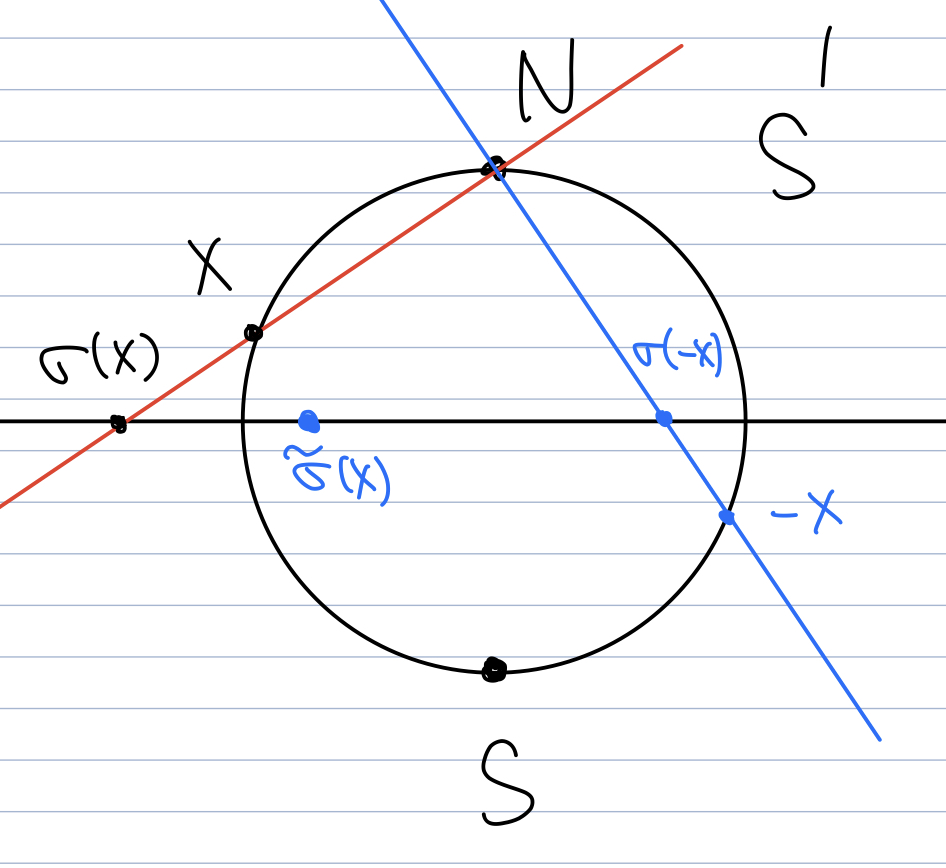
\includegraphics[width=.5\linewidth]{img/problem_1_7.jpeg}
    \caption{Problem 1-7}
    \label{fig:problem_1_7}
  \end{figure}
  $ $
  \begin{enumerate}[label=(\alph*)]
    \item 
      This is trivial from a basic trigonometry argument using the triangles $N, (0, \cdots, 0, x^{n + 1}), (x^1, \cdots, x^{n + 1})$ and $N, (0, \cdots, 0), \sigma(x^1, \cdots, x^{n + 1})$.
    \item
      $\sigma \circ \sigma^{-1}$ and $\sigma^{-1} \circ \sigma$ are both the identity maps, so $\sigma$ is bijective and $\sigma^{-1}$ is its inverse.
    \item
      Computation shows that $\tilde{\sigma} \circ \sigma^{-1}: S^n \setminus \{ N, S \} \rightarrow S^n \setminus \{ N, S \}$ sends $(u^1, \cdots, u^n)$ to $(u^1, \cdots, u^n) / \abs{u}^2$.
      As $\abs{u} \ne 0$ in the domain, this map is well-defined and clearly smooth.
      By Proposition 1.17(a), these two charts determine a unique smooth structure.
    \item
      $\phi_i, \sigma, \tilde{\sigma}$ are all smooth functions of subsets of Euclidean spaces, so transition maps are always smooth.
      By Proposition 1.17(b), the smooth structure determined by $\sigma, \tilde{\sigma}$ is the same as the one defined in Example 1.31.
  \end{enumerate}
\end{proof}

\begin{customprob}{1-12(Proof of Proposition 1.45)}
  Suppose $M_1, \cdots, M_k$ are smooth manifolds and $N$ is a smooth manifold with boundary.
  Then $M_1 \times \cdots \times M_k \times N$ is a smooth manifold with boundary, and $\partial (M_1 \times \cdots \times M_k \times N) = M_1 \times \cdots \times M_k \times \partial N$.
\end{customprob}

\begin{proof}
  By Example 1.34, $M_1 \times \cdots \times M_k$ is a smooth manifold.
  Thus it suffices to show that $M \times N$ is a smooth manifold with boundary if $M$ is a smooth manifold and $N$ is a smooth manifold with boundary.
  Let $m, n$ be the dimensions of $M, N$.

  First, we show that $M \times N$ is a topological manifold with boundary and $\partial(M \times N) = M \times \partial N$.
  Let $(p, q) \in M \times N$.
  Then $p \in M$, so there exists a chart $(U, \phi)$ such that $p \in U$ and $\hat{U} = \phi(U) \subset \mathbb{R}^m$.

  \begin{itemize}
    \item
      Suppose $q \in \Int N$.
      Then there exists a chart $(V, \psi)$ such that $\hat{V} = \psi(V) \subset \mathbb{R}^n$.
      $\phi \times \psi$ is a homeomorphism between $U \times V$ and $\hat{U} \times \hat{V} \subset \mathbb{R}^m \times \mathbb{R}^n = \mathbb{R}^{m + n}$.
      Thus $(U \times V, \phi \times \psi)$ is a chart for $(p, q)$.
    \item
      Suppose $q \in \bd N$.
      Then there exists a chart $(V, \psi)$ such that $\hat{V} = \psi(V) \subset \mathbb{H}^n$ and $\psi(q) \in \partial \mathbb{H}^n$.
      $\phi \times \psi$ is a homeomorphism between $U \times V$ and $\hat{U} \times \hat{V} \subset \mathbb{R}^m \times \mathbb{H}^n = \mathbb{H}^{m + n}$.
      Moreover, $(\phi \times \psi)(p, q) = (\phi(p), \psi(q)) \in \mathbb{R}^m \times \mathbb{H}^n = \mathbb{H}^{m + n}$.
      Thus $(U \times V, \phi \times \psi)$ is a boundary chart for $(p, q)$.
  \end{itemize}

  Therefore, $M \times N$ is a topological manifold with boundary and $\partial (M \times N) = M \times (\partial N)$.

  Let $\mathcal{A}_M, \mathcal{A}_N$ be the smooth structures of $M, N$.
  Define $\mathcal{A}_{M \times N} = \{ (U \times V, \phi \times \psi) \mid (U, \phi) \in \mathcal{A}_M, (V, \psi) \in \mathcal{A}_N \}$.
  Then $\mathcal{A}_{M \times N}$ is an atlas because we showed earlier that each $(U \times V, \phi \times \psi)$ is a chart.
  Let $(U_1 \times V_1, \phi_1 \times \psi_1), (U_2 \times V_2, \phi_2 \times \psi_2) \in \mathcal{A}_{M \times N}$.
  Then $(\phi_2 \times \psi_2) \circ (\phi_1 \times \psi_1)^{-1} = (\phi_2 \circ \phi_1^{-1}) \times (\psi_2 \circ \psi_1^{-1})$ is a smooth map from $(\phi_1 \times \psi_1)(U_1 \times V_1)$ into $(\phi_2 \times \psi_2)(U_2 \times V_2)$.
  Thus every pair of charts in $\mathcal{A}_{M \times N}$ is smoothly compatible.
  In other words, $\mathcal{A}_{M \times N}$ is a smooth atlas.

  On the other hand, $\mathcal{A}_{M \times N}$ must be maximal because the restriction of any smoothly compatible chart to $M, N$ gives a smoothly compatible chart, which must belong to $\mathcal{A}_M, \mathcal{A}_N$, respectively.
  Thus $M \times N$ is a smooth manifold with boundary.
\end{proof}


\section{Chapter 2: Smooth Maps}
\begin{customexer}{2.1}
  Let $M$ be a smooth manifold with or without boundary.
  Show that pointwise multiplication turns $C^{\infty}(M)$ into a commutative ring and a commutative and associative algebra over $\mathbb{R}$.
\end{customexer}

\begin{proof}
  $ $
  \begin{itemize}
    \item
      The constant map $f(p) = 0$ is clearly in $C^{\infty}(M)$ and it is the additive identity.
    \item
      The constant map $f(p) = 1$ is clearly in $C^{\infty}(M)$ and it is the multiplicative identity.
    \item
      Let $f \in C^{\infty}(M), g \in C^{\infty}(M)$.
      Let $p \in M$ and $(\phi, U)$ be a smooth chart for $p$.
      Then $f \circ \phi^{-1}$ and $g \circ \phi^{-1}$ are both smooth(Exercise \ref{ex_2_3}), real-valued maps defined on an open subset of $\mathbb{R}^n$.
      Thus $f + g$ is in $C^{\infty}(M)$ 
      Moreover, $f + g = g + f$ because addition in $\mathbb{R}$ is commutative.
    \item
      Let $f, g, h \in C^{\infty}(M)$.
      Let $p \in M$ and $(\phi, U)$ be a smooth chart for $p$.
      Then $f \circ \phi^{-1}$ and $g \circ \phi^{-1}$ are both smooth(Exercise \ref{ex_2_3}), real-valued maps defined on an open subset of $\mathbb{R}^n$.
      Therefore, $fg$ is in $C^{\infty}(M)$
      Moreover, $fg = gf$ and $(fg)h = f(gh)$ because multiplication in $\mathbb{R}$ is commutative and associative.
    \item
      Let $c \in \mathbb{R}, f \in C^{\infty}(M)$.
      Then $cf$ can be seen as $fg$ where $g$ is the constant function whose value is $c$.
      As shown above, $cf \in C^{\infty}(M)$.
  \end{itemize}
\end{proof}

\begin{customexer}{2.2}
  Let $U$ be an open submanifold of $\mathbb{R}^n$ with its standard smooth manifold structure.
  Show that a function $f: U \rightarrow \mathbb{R}^k$ is smooth in the sense just defined if and only if it is smooth in the sense of ordinary calculus.
  Do the same for an open submanifold with boundary in $\mathbb{H}^n$.
\end{customexer}

\begin{proof}
  $f$ is smooth in the sense just defined if and only if $f^{-1} \circ \Id^{-1}$ is smooth in the sense of ordinary calculus.
  Since $f^{-1} \circ \Id^{-1} = f^{-1}$, $f^{-1} \circ \Id^{-1}$ is smooth in the sense of ordinary calculus if and only if $f^{-1}$ is smooth in the sense of ordinary calculus.
\end{proof}

\begin{customexer}{2.3}\label{ex_2_3}
  Let $M$ be a smooth manifold with or without boundary, and suppose $f: M \rightarrow \mathbb{R}^k$ is a smooth function.
  Show that $f \circ \phi^{-1}: \phi(U) \rightarrow \mathbb{R}^k$ is smooth for every smooth chart $(U, \phi)$ for $M$.
\end{customexer}

\begin{proof}
  Let $\phi(x) \in \phi(U)$.
  Since $f$ is smooth, there exists $(V, \psi)$ such that $f \circ \psi^{-1}: \psi(V) \rightarrow \mathbb{R}^k$ is smooth and $x \in V$.
  Let $W = U \cap V$.
  Then $f \circ \psi^{-1}: \psi(W) \rightarrow \mathbb{R}^k$ is smooth and $\psi \circ \phi^{-1}: \phi(W) \rightarrow \psi(W)$ is a diffeomorphism where $\phi(W)$ is a neighborhood of $W$.
  Then the restriction of $f \circ \psi^{-1}$ to $\phi(W)$ is identical to $(f \circ \psi^{-1}) \circ (\psi \circ \phi^{-1})$.
  Since he composition of a smooth function is smooth, $f \circ \psi^{-1}$ is smooth.
\end{proof}


\section{Chapter 3: Tangent Vectors}
\subsection{Exercises}
\begin{customexer}{3.5(Proof of Lemma 3.4)}
  Suppose $M$ is a smooth manifold with or without boundary, $p \in M, v \in T_pM$, and $f, g \in C^{\infty}(M)$.
  \begin{enumerate}[label=(\alph*)]
    \item 
      If $f$ is a constant function, then $vf = 0$.
    \item
      If $f(p) = g(p) = 0$, then $v(fg) = 0$.
  \end{enumerate}
\end{customexer}

\begin{proof}
  $ $
  \begin{enumerate}[label=(\alph*)]
    \item
      Let $h$ be the constant function that always takes the value 1.
      Then $f(p) = ch(p)$ for some $c \in \mathbb{R}$.
      Then $v(ff) = f(p)vf + f(p)vf$, so $c^2v(h) = c^2v(h) + c^2v(h)$.
      Therefore, $c^2v(h) = 0$, so $cv(h) = 0$.
      Since $v$ is linear, this implies $0 = v(ch) = v(f)$, so $v(f) = 0$.
    \item
      $v(fg) = f(p)vg + g(p)vf = 0 + 0 = 0$.
  \end{enumerate}
\end{proof}

\begin{customexer}{3.7(Proof of Proposition 3.6)}
  Let $M, N$, and $P$ be smooth manifolds with or without boundary, let $F: M \rightarrow N$ and $G: N \rightarrow P$ be smooth maps, and let $p \in M$.
  \begin{enumerate}[label=(\alph*)]
    \item
      $dF_p:T_pM \rightarrow T_{F(p)}N$ is linear.
    \item
      $d(G \circ F)_p = dG_{F(p)} \circ dF_p: T_pM \rightarrow T_{G \circ F(p)} P$.
    \item
      $d(\Id_M)_p = \Id_{T_pM}: T_pM \rightarrow T_pM$.
    \item
      If $F$ is a diffeomorphism, then $dF_p: T_pM \rightarrow T_{F(p)}N$ is an isomorphism, and $(dF_p)^{-1} = d(F^{-1})_{F(p)}$.
  \end{enumerate}
\end{customexer}

\begin{proof}
  \begin{enumerate}[label=(\alph*)]
    \item
      $\forall v, w \in T_pM, \forall c \in \mathbb{R}, \forall f \in C^{\infty}(N)$,
      \begin{align*}
        dF_p(cv + w)(f)
          &= (cv + w)(f \circ F) \\
          &= (cv)(f \circ F) + w(f \circ F) \\
          &= c(v(f \circ F)) + w(f \circ F) \\
          &= c(dF_p(v)(f)) + dF_p(w)(f) \\
          &= (cdF_p(v))(f) + dF_p(w)(f) \\
          &= (cdF_p(v) + dF_p(w))(f).
      \end{align*}
      Therefore, $dF_p(cv + w) = cdF_p(v) + dF_p(w)$.
    \item
      $\forall v \in T_pM, f \in C^{\infty}(P)$,
      \begin{align*}
        d(G \circ F)_p(v)(f)
          &= v(f \circ (G \circ F)) \\
          &= v((f \circ G) \circ F) \\
          &= (dF_p(v))(f \circ G) \\
          &= (dG_{F(p)}(dF_p(v)))(f) \\
          &= ((dG_{F(p)} \circ dF_p)(v))(f) \\
      \end{align*}
      Therefore, $d(G \circ F)_p = dG_{F(p)} \circ dF_p$.
    \item
      $\forall v \in T_p(M), \forall f \in C^{\infty}(M)$,
      \begin{align*}
        d(\Id_M)_p(v)(f)
          &= v(f \circ \Id_M) \\
          &= v(f).
      \end{align*}
      Therefore, $d(\Id_M)_p(v) = v$, so $d(\Id_M)_p = \Id_{T_pM}$.
    \item
      $F^{-1}$ exists and it is a smooth map since $F$ is a diffeomorphism.
      By combining (b) and (c), we obtain $dF_p$ and $dF^{-1}_{F(p)}$ are the inverse of each other.
      Therefore, $dF_p$ is an isomorphism.
  \end{enumerate}
\end{proof}

\subsection{Problems}

\begin{customprob}{3-1}
  Suppose $M$ and $N$ are smooth manifolds with or without boundary, and $F: M \rightarrow N$ is a smooth map.
  Show that $dF_p: T_pM \rightarrow T_{F(p)}N$ is the zero map for each $p \in M$ if and only if $F$ is constant on each component of $M$.
\end{customprob}

\begin{proof}
  \todo[inline,caption={}]{
    Show the other direction.
  }
  Suppose $F$ is constant on each component of $M$.
  Let $p \in M$.
  Choose a chart $(U, \phi) \in \mathcal{A}_M$ such that $p \in U$.
  Then $F \circ \phi^{-1}$ is constant in a neighborhood around $\phi(p)$.
  For any $i$,
  \begin{align*}
    dF_p(\frac{\partial}{\partial x^i}\vert_p)(f)
      &= \frac{\partial}{\partial x^i}\vert_p(f \circ F) \\
      &= \frac{\partial}{\partial x^i}\vert_{\phi(p)}(f \circ F \circ \phi^{-1}) \\
      &= 0
  \end{align*}
  because $f \circ F \circ \phi^{-1}$ is constant in a neighborhood around $\phi(p)$.
  By Proposition 3.15, $\partial / \partial x^i\vert_p$ form a basis for $T_pM$.
  Since $dF_p$ sends each basis element to 0, $dF_p = 0$.
\end{proof}

\begin{customprob}{3-2(Proof of Proposition 3.14)}\label{problem_3_2}
  Let $M_1, \cdots, M_k$ be smooth manifolds, and for each $j$, let $\pi_j: M_1 \times \cdots \times M_k \rightarrow M_j$ be the projection onto the $M_j$ factor.
  For any point $p = (p_1, \cdots, p_k) \in M_1 \times \cdots \times M_k$, the map
  \begin{align*}
    \alpha: T_p(M_1 \times \cdots \times M_k) \rightarrow T_{p_1}M_1 \oplus \cdots \oplus T_{p_k}M_k
  \end{align*}
  defined by
  \begin{align*}
    \alpha(v) = (d(\pi_1)_p(v), \cdots, d(\pi_k)_p(v))
  \end{align*}
  is an isomorphism.
  The same is true if one of the spaces $M_i$ is a smooth manifold with boundary.
\end{customprob}

\begin{proof}
  It suffices to show this for the case that $k = 2$ because the results extend to arbitrary $k$ by induction.
  Let $\mathcal{A}_{M_1}, \mathcal{A}_{M_2}, \mathcal{A}_{M_1 \times M_2}$ be the smooth structures of $M_1, M_2, M_1 \times M_2$.

  We first define a lot of notations.
  \begin{itemize}
    \item
      Let $d_1, d_2$ denote the dimensions of $M_1, M_2$ and let $d = d_1 + d_2$ denote the dimension of $M_1 \times M_2$.
    \item
      Let $p = (p_1, p_2) \in M_1 \times M_2$ be given.
      Choose $(U, \phi = (x^i)) \in \mathcal{A}_{M_1}, (V, \psi = (y^i)) \in \mathcal{A}_{M_2}$ with $p_1 \in U$ and $p_2 \in V$.
      Let $q_1 = \phi(p_1), q_2 = \psi(p_2), q = q_1 \times q_2$.
    \item
      $(U \times V, (z^i)) \in \mathcal{A}_{M_1 \times M_2}$ and $(p_1, p_2) \in U \times V$ where $(z^i) = \phi \times \psi$.
      More specifically, $z^i = x^i \circ \pi_1$ for $1 \leq i \leq d_1$ and $z^i = y^i \circ \pi_2$ for $d_1 + 1 \leq i \leq d_1 + d_2$.
  \end{itemize}
  Note that we use $x^i, y^i, z^i, \pi_1$ to mean two different things in this solution: 
  \begin{itemize}
    \item
      $x^i$ is either the $i$th coordinate function of $\phi$ or the $i$th projection map $\mathbb{R}^{d_1} \rightarrow \mathbb{R}$.
    \item
      $y^i$ is either the $i$th coordinate function of $\psi$ or the $i$th projection map $\mathbb{R}^{d_2} \rightarrow \mathbb{R}$.
    \item
      $z^i$ is either the $i$th coordinate function of $\phi \times \psi$ or the $i$th projection map $\mathbb{R}^{d_1 + d_2} \rightarrow \mathbb{R}$.
    \item
      $\pi_1$ is either the projection map $M_1 \times M_2 \rightarrow M_1$ or the projection map $\mathbb{R}^{d_1 + d_2} \rightarrow \mathbb{R}^{d_1}$.
    \item
      $\pi_2$ is either the projection map $M_1 \times M_2 \rightarrow M_2$ or the projection map $\mathbb{R}^{d_1 + d_2} \rightarrow \mathbb{R}^{d_2}$.
  \end{itemize}

  By Proposition 3.15, $\{ \partial / \partial x^1 \vert_{p_1}, \cdots, \partial / \partial x^{d_1} \vert_{p_1} \}, \{ \partial / \partial y^1 \vert_{p_2}, \cdots, \partial / \partial y^{d_2} \vert_{p_2} \}, \{ \partial / \partial z^1 \vert_{p}, \cdots, \partial / \partial z^{d_1 + d_2} \vert_{p} \}$ form bases for $T_{p_1}M_1, T_{p_2}M_2, T_p(M_1 \times M_2)$.

  $\alpha(\partial / \partial z^1 \vert_p) = (d(\pi_1)_p(\partial/\partial z^1\vert_p), d(\pi_2)_p(\partial/\partial z^1\vert_p))$.
  We claim that $d(\pi_1)_p(\partial / \partial z^1 \vert_p) = \partial / \partial x^1 \vert p_1$.

  \begin{align*}
    d(\pi_1)_p(\partial / \partial z^1 \vert_p)(f)
      &= d(\pi_1)_p(d(\phi^{-1} \times \psi^{-1})_q)(\frac{\partial}{\partial z^1}\vert_q) (f)\\
      &= (d(\pi_1)_p \circ d(\phi^{-1} \times \psi^{-1})_q)(\frac{\partial}{\partial z^1}\vert_q) (f)\\
      &= d(\pi_1 \circ (\phi^{-1} \times \psi^{-1})_q)(\frac{\partial}{\partial z^1}\vert_q) (f)\\
      &= \lim_{h \rightarrow 0} \frac{(f \circ \pi_1 \circ (\phi^{-1} \times \psi^{-1}))(q + e_1h) - (f \circ \pi_1 \circ (\phi^{-1} \times \psi^{-1}))(q)}{h} \\
      &= \lim_{h \rightarrow 0} \frac{(f \circ \pi_1)(\phi^{-1}(q_1 + e_1h), p_2) - (f \circ \pi_1)(p)}{h} \\
      &= \lim_{h \rightarrow 0} \frac{f(\phi^{-1}(q_1 + e_1h)) - f(p_1)}{h} \\
      &= \lim_{h \rightarrow 0} \frac{f(\phi^{-1}(q_1 + e_1h)) - f(\phi^{-1}(q_1))}{h} \\
      &= (\frac{\partial}{\partial x^1}\vert_{q_1})(f \circ \phi^{-1}) \\
      &= d(\phi^{-1})_{q_1}(\frac{\partial}{\partial x^1}\vert_{q_1})(f) \\
      &= (\frac{\partial}{\partial x^1}\vert_{p_1})(f).
  \end{align*}

  The same result can be shown for the other combinations of $\pi_1, \pi_2$ and $z^1, \cdots, z^{d_1 + d_2}$.
  For any $c_1, \cdots, c_{d_1 + d_2} \in \mathbb{R}$,
  \begin{align*}
    \alpha(\sum_{i=1}^{d_1 + d_2} c_{i}\frac{\partial}{\partial z^{i}}\vert_p)
      &= \sum_{i=1}^{d_1 + d_2} c_i\alpha(\frac{\partial}{\partial z^{i}}\vert_p) \\
      &= \sum_{i=1}^{d_1 + d_2} c_i(d(\pi_1)_p\frac{\partial}{\partial z^{i}}\vert_p, d(\pi_2)_p\frac{\partial}{\partial z^i}\vert_p) \\
      &= \sum_{i=1}^{d_1} c_i(d(\pi_1)_p\frac{\partial}{\partial z^{i}}\vert_p, d(\pi_2)_p\frac{\partial}{\partial z^i}\vert_p) 
         + \sum_{i=d_1 + 1}^{d_2} c_i(d(\pi_1)_p\frac{\partial}{\partial z^{i}}\vert_p, d(\pi_2)_p\frac{\partial}{\partial z^i}\vert_p) \\
      &= \sum_{i=1}^{d_1} c_i(\frac{\partial}{\partial x^i} \vert_{p_1}, 0)
         + \sum_{i=1}^{d_2} c_{d_1 + i}(0, \frac{\partial}{\partial y^i} \vert_{p_2}) \\
      &= (c_1\frac{\partial}{\partial x^1}\vert_{p_1} + \cdots + c_{d_1}\frac{\partial}{\partial x^{d_1}}\vert_{p_1},
          c_{d_1 + 1}\frac{\partial}{\partial y^{1}}\vert_{p_2} + \cdots + c_{d_1 + d_2}\frac{\partial}{\partial y^{d_2}}\vert_{p_2}).
  \end{align*}

  Therefore, $\alpha$ is bijective.
\end{proof}


\section{Chapter 4: Submersions, Immersions, and Embeddings}
\begin{customthm}{4.1}
  Suppose $F: M \rightarrow N$ is a smooth map and $p \in M$.
  If $dF_p$ is surjective, then $p$ has a neighborhood $U$ such that $F\vert_U$ is a submersion.
  If $dF_p$ is injective, then $p$ has a neighborhood $U$ such that $F\vert_U$ is an immersion.
\end{customthm}

\begin{proof}
  Let $(U, \phi)$ be a chart containing $p$ and $(V, \psi)$ be a chart containing $F(p)$.
  We may assume $F(U) \subset V$.
  It suffices to show that if the Jacobian of $F$ with respect to $(U, \phi)$ is full rank at $p$, then it is full rank in some neighborhood of $p$ contained in $U$.
  Example 1.28 in the textbook shows that the set of full rank matrices is an open subset of $M(m \times n, \mathbb{R})$.
  We will use the notation $J\vert_{q}$ to denote the Jacobian of $F$ with respect to $(U, \phi)$ at $q \in U$.
  Then $J\vert_{p}$ is an element of an open subset of $M(m \times n, \mathbb{R})$.
  Each entry of $J\vert_{q}$ is of the from $\frac{\partial}{\partial x^i}(\psi^j \circ F \circ \phi)(\phi(q))$ where each $(\frac{\partial}{\partial x^i}(\psi^j \circ F \circ \phi)) \circ \phi$ is a smooth function.
  Therefore, there exists a neighborhood of $p$ such that the Jacobian matrix of $F$ with respect to $(U, \phi)$ is full rank.
\end{proof}

\begin{customexer}{4.3(Verification of Example 4.2)}
  Verify the following claims:
  \begin{enumerate}[label=(\alph*)]
    \item
      Suppose $M_1, \cdots, M_k$ are smooth manifolds.
      Then each of the projection maps $\pi_i: M_1 \times \cdots \times M_k \rightarrow M_i$ is a smooth submersion.
    \item
      If $\gamma: J \rightarrow M$ is a smooth curve in a smooth manifold $M$ with or without boundary, then $\gamma$ is a smooth immersion if and only if $\gamma'(t) \ne 0$ for all $t \in J$.
  \end{enumerate}
\end{customexer}

\begin{proof}
   $ $
  \begin{enumerate}[label=(\alph*)]
    \item
      Let $d_1, \cdots, d_k$ denote the dimensions of $M_1, \cdots, M_k$, respectively.
      Let $M = M_1 \times \cdots \times M_k$.

      (\ref{problem_2_2}) implies that $\pi_i$ is smooth for each $i$ by setting $F = \Id: M \rightarrow M$.
      Let $p = (p_1, \cdots, p_k) \in M$.
      Thus it suffices to show that the dimension of $d(\pi_i)_p(T_p(M))$ is the same as the dimension of $T_{p_i}(M_i)$.

      By Proposition 3.12, $\dim(T_p(M)) = \sum d_i$.
      Since the $\alpha$ defined in (\ref{problem_3_2}) is an isomorphism,
      \begin{equation}\label{exercise_4_3_eq_1}
        \dim(d(\pi_1)_p(T_p(M)) \oplus \cdots \oplus d(\pi_k)_p(T_p(M))) = \dim(T_p(M)) = \sum d_i.
      \end{equation}

      However, for each $i$, $d(\pi_i)_p(T_p(M)) \subset T_{p_i}M_i$.
      Thus $\dim(d(\pi_i)_p(T_p(M))) \leq \dim(T_{p_i}M_i) = d_i$.
      By (\ref{exercise_4_3_eq_1}), $\dim(d(\pi_i)_p(T_p(M))) = \dim(T_{p_i}M_i)$.
    \item
      $\gamma$ is a smooth immersion if and only if $d\gamma_t: T_tJ \rightarrow T_{\gamma(t)}M$ is injective for each $t \in J$.
      Since each $T_tJ$ is a 1-dimensional vector space spanned by $d/dt\vert_t$, $d\gamma_t$ is injective if and only if $d\gamma_t$ sends the basis element to a nonzero element.
      Finally, $\gamma'(t) = d\gamma(d/dt\vert_{t})$.
      Therefore, $\gamma$ is a smooth immersion if and only if $\gamma'(t) \ne 0$ for all $t \in J$.
  \end{enumerate}
\end{proof}

\begin{customexer}{4.4}
  Show that a composition of smooth submersions is a smooth submersion, and a composition of smooth immersions is a smooth immersion.
  Give a counterexample to show that a composition of maps of constant rank need not have constant rank.
\end{customexer}

\begin{proof}
  Let $M, N, L$ be smooth manifolds with or without boundary, and $F: M \rightarrow N, G: N \rightarrow L$ be given.
  If $F, G$ are submersions, $dF_p$ and $dG_{F(p)}$ are surjective for each $p$.
  Then $d(G \circ F)_p = dG_{F(p)} \circ dF_p$ is surjective for each $p$ by (\ref{proof_prop_3_6}).
  Thus a composition of smooth submersions is a smooth submersion.
  By the exact same argument, a composition of smooth immersions is a smooth immersion.
  \todo[inline,caption={}]{
    Counterexample?
  }
\end{proof}

\begin{customthm}{4.5}
  Suppose $M$ and $N$ are smooth manifolds, and $F: M \rightarrow N$ is a smooth map.
  If $p \in M$ is a point such that $dF_p$ is invertible, then there are connected neighborhoods $U_0$ of $p$ and $V_0$ of $F(p)$ such that $F\vert_{U_0}: U_0 \rightarrow V_0$ is a diffeomorphism.
\end{customthm}

\begin{proof}
  Since $dF_p$ is invertible, $\dim(T_pM) = \dim(T_{F(p)}N)$.
  Let $n = \dim(T_pM)$.
  By (\ref{proposition_3_10}), $n$ is the dimension of $M$ and $N$.
  Let $(U, \phi), (V, \psi)$ be smooth charts containing $p, F(p)$, respectively, such that $\phi(p) = \psi(F(p)) = 0 \in \mathbb{R}^n$ and $F(U) \subset V$.
  Let $\hat{F} = \psi \circ F \circ \phi^{-1}$.
  Then $\hat{F}$ is a smooth map from an open subset $\hat{U} \subset \mathbb{R}^n$ into an open subset $\hat{V} \subset \mathbb{R}^n$.
  Then $d\hat{F}\vert_0 = d\psi_{F(p)} \circ dF_p \circ d\phi^{-1}_0$.
  Each function on the right hand side is bijective, so $d\hat{F}\vert_0$ is bijective.
  Since the differential of a smooth map between Euclidean spaces coincides with the total derivative of the map, we may apply the ordinary inverse function theorem.
  Thus there exist connected open subsets $\hat{U}_0 \subset \hat{U}$ and $\hat{V}_0 \subset \hat{V}$ both containing 0 such that $\hat{F}$ is a diffeomorphism from $\hat{U}_0$ to $\hat{V}_0$.
  Since $\phi$ and $\psi$ are homeomorphisms, $U_0$ and $V_0$ are connected neighborhoods of $p$ and $F(p)$ respectively.
  Finally, since $F = \psi^{-1} \circ \hat{F} \circ \phi$, $F$ is a diffeomorphism from $U_0$ to $V_0$.
\end{proof}


\section{Appendix A: Review of Topology}
\begin{customexer}{A.18(Proof of Proposition A.17)}\label{exercise_a_18}
  Let $X$ be a topological space and let $S$ be a subspace of $X$.
  \begin{enumerate}[label=(\alph*)]
    \item 
    \item 
    \item 
    \item 
    \item 
    \item 
      If $\mathcal{B}$ is a basis for the topology of $X$, then $\mathcal{B}_S = \{ B \cap S \mid B \in \mathcal{B} \}$ is a basis for the subspace topology on $S$.
    \item 
      If $X$ is Hausdorff, then so is $S$.
    \item 
      If $X$ is first-countable, then so is $S$.
    \item 
      If $X$ is second-countable, then so is $S$.
  \end{enumerate}
\end{customexer}

\begin{proof}
  $ $
  \begin{enumerate}[label=(\alph*)]
    \item 
    \item 
    \item 
    \item 
    \item 
    \item 
      The union of $B \cap S$ is $S$.
      Let $U \cap S$ be an open subset of $S$ where $U$ is open in $X$, and $x \in U \cap S$.
      Then there exists $B \in \mathcal{B}$ such that $x \in B \subset U$ since $\mathcal{B}$ is a basis.
      Therefore, $x \in B \cap S \subset U \cap S$ with $B \cap S \in \mathcal{B}_S$.
    \item 
      Let $x \ne y \in S$.
      There exist two disjoint open sets $U, V$ of $X$ containing $x, y$, respectively.
      Then $U \cap S$ and $V \cap S$ are disjoint open sets of $X$ containing $x, y$, respectively.
    \item 
    \item 
      Let $\mathcal{B}$ be a countable basis of $X$.
      Then $\{ B \cap S \mid B \in \mathcal{B} \}$ is a countable basis of $S$ by (f).
  \end{enumerate}
\end{proof}

\begin{customexer}{A.24(Proof of Proposition A.23)}\label{exercise_a_24}
  Suppose $X_1, \cdots, X_k$ are topological spaces, and let $X_1 \times \cdots \times X_k$ be their product space.
  \begin{enumerate}[label=(\alph*)]
    \item
      CHARACTERISTIC PROPERTY: If $B$ is a topological space, a map $F: B \rightarrow X_1 \times \cdots \times X_k$ is continuous if and only if each of its component functions $F_i = \pi_i \circ F: B \rightarrow X_i$ is continuous.
  \end{enumerate}
\end{customexer}

\begin{proof}
  $ $
  \begin{enumerate}[label=(\alph*)]
    \item
      Suppose $F$ is continuous.
      Since $\pi_i$ is continuous by (c) and the composition of continuous functions is continuous, $\pi_1 \circ F$ is continuous.
      Suppose each component function is continuous.
      Let $B_1 \times \cdots \times B_k$ be a basis element of $X_1 \times \cdots \times X_k$.
      \begin{align*}
        F^{-1}(B_1 \times \cdots \times B_k)
          &= F^{-1}(\cap_{i=1}^{k} \pi_i^{-1}(B_1 \times \cdots \times B_k)) \\
          &= \cap_{i=1}^{k} F^{-1}(\pi_i^{-1}(B_1 \times \cdots \times B_k)) \\
          &= \cap_{i=1}^{k} (\pi_i \circ F)^{-1}(B_1 \times \cdots \times B_k).
      \end{align*}
      Since the intersection of finitely many open sets is open, $F$ is continuous.
  \end{enumerate}
\end{proof}


\section{Appendix B: Review of Linear Algebra}
\begin{customexer}{B.49}
  Two norms $\abs{\cdot}_1$ and $\abs{\cdot}_2$ on a vector space $V$ are said to be equivalent if there are positive constants $c, C$ such that
  \begin{align*}
    c\abs{v}_1 \leq \abs{v}_2 \leq C\abs{v}_1
  \end{align*}
  for all $v \in V$.
  Show that equivalent norms determine the same topology.
\end{customexer}

\begin{proof}
  Such a relation is symmetric for $c\abs{v}_1 \leq \abs{v}_2 \leq C\abs{v}_1$ implies $(1/C)\abs{v}_2 \leq \abs{v}_1 \leq (1/c)\abs{v}_2$.
  Let $\mathcal{T}_1, \mathcal{T}_2$ be the topologies induced by $\abs{\cdot}_1, \abs{\cdot}_2$.
  It suffices to show that $\forall v \in V, \forall U \in \mathcal{T}_2, (v \in U \implies \exists r > 0, B_1(v, r) \subset U)$ where $B_1(v, r)$ is the open ball centered at $v$ with the radius $r$ using the $\abs{\cdot}_1$.
  Since $v \in U$ and $U$ is open, $\exists r > 0$ such that $B_2(v, r) \subset U$.
  Then for any $w \in V$, $\abs{v - w}_1 \leq \abs{v - w}_2 / c$, so $B_1(v, r / c) \subset B_2(v, r)$.
\end{proof}


\section{Appendix C: Review of Calculus}
\begin{customexer}{C.1}
  Suppose that $F: U \rightarrow W$ is differentiable at $a \in U$. Show that the linear map satisfying

  \begin{align*}
    \lim_{v \rightarrow 0} \frac{\abs{F(a + v) - F(a) - Lv}}{\abs{v}} = 0
  \end{align*}

  is unique.
\end{customexer}

\begin{proof}
  Let $L, L'$ be two such linear maps.
  \begin{align*}
    \lim_{v \rightarrow 0} \frac{\abs{Lv - L'v}}{\abs{v}}
      &= \lim_{v \rightarrow 0} \frac{\abs{(F(a + v) - F(a) - L'v) - (F(a + v) - F(a) - Lv)}}{\abs{v}} \\
      &= \lim_{v \rightarrow 0} \frac{\abs{F(a + v) - F(a) - Lv}}{\abs{v}} + \lim_{v \rightarrow 0} \frac{\abs{F(a + v) - F(a) - L'v}}{\abs{v}} \\
      &= 0 + 0 = 0.
  \end{align*}
  If $L \ne L'$, $(L - L')v_0 \ne 0$ for some $v_0$.
  Then $\lim_{v \rightarrow 0} \frac{\abs{Lv - L'v}}{\abs{v}} = \lim_{h \rightarrow 0} \frac{\abs{L(hv_0) - L'(hv_0)}}{\abs{hv_0}} = \frac{\abs{(L - L')v_0}}{\abs{v_0}} \ne 0$.
  This is a contradiction, so $L = L'$.
\end{proof}



\section{Dictionary}
\subsection{Topological Manifolds}

\begin{defn}[Topological Manifold]
  A \textit{topological $n$-manifold} is a Hausdorff, second-countable topological space each point of which has a neighborhood that is homeomorphic to an open subset $\mathbb{R}^n$.
\end{defn}

\begin{defn}[Coordinates]
  Let $M$ be a topological $n$-manifold.
  Let $U$ be an open subset of $M$, $\hat{U}$ be an open subset of $\mathbb{R}^n$, $\phi: U \rightarrow \hat{U}$ be a homeomorphism.
  \begin{itemize}
    \item
      The pair $(U, \phi)$ is called a \textit{coordinate chart} or a \textit{chart}.
    \item
      $U$ is called a \textit{coordinate domain} or a \textit{coordinate neighborhood} and $\phi$ is called a \textit{coordinate map}.
    \item
      If $\phi(U)$ is an open ball in $\mathbb{R}^n$, $U$ is called a \textit{coordinate ball}.
    \item
      If $\phi(U)$ is an open cube in $\mathbb{R}^n$, $U$ is called a \textit{coordinate cube}.
  \end{itemize}
\end{defn}

\begin{defn}[Atlas]
  Let $M$ be a topological $n$-manifold.
  An \textit{atlas for $M$} is a collection of charts $(U_{\alpha}, \phi_{\alpha})$ such that $M = \bigcup_{\alpha} U_{\alpha}$.
\end{defn}

\begin{defn}[Transition Map]
  Let $M$ be a topological $n$-manifold and $(U, \phi), (V, \psi)$ be coordinate charts such that $U \cap V \ne \emptyset$.
  $\psi \circ \phi^{-1}: \phi(U \cap V) \mapsto \psi(U \cap V)$ is called a \textit{transition map} from $\phi$ to $\psi$.
\end{defn}

\begin{defn}[Closed Upper Half-Space]
  $\mathbb{H}^n = \{ (x^1, \cdots, x^n) \in \mathbb{R}^n \mid x^n \geq 0 \}$, and $\partial \mathbb{H}^n = \{ (x^1, \cdots, x^n) \in \mathbb{R}^n \mid x^n = 0 \}$.
\end{defn}

\begin{defn}[Manifold With Boundary]
  Let $M$ be a second-countable Hausdorff space and fix $n$.
  Suppose that for every $p \in M$, one of the following conditions is satisfied:
  \begin{enumerate}
    \item
      There exists a neighborhood $U$ of $p$ and a homeomorphism $\phi:U \rightarrow \hat{U}$ where $\hat{U}$ is an open subset of $\mathbb{R}^n$.
      $p$ is called an \textit{interior point} and $(U, \phi)$ is called an \textit{interior chart}.
    \item
      There exists a neighborhood $U$ of $p$ and a homeomorphism $\phi:U \rightarrow \hat{U}$ where $\hat{U}$ is an open subset of $\mathbb{H}^n$ with $\hat{U} \cap \partial \mathbb{H}^n \ne \emptyset$.
      $p$ is called a \textit{boundary point} and $(U, \phi)$ is called a \textit{boundary chart}.
  \end{enumerate}
  Then $M$ is called an \textit{$n$-dimensional topological manifold with boundary}.
  Note that every topological manifold is a topological manifold with boundary.
\end{defn}


\subsection{Smooth Manifolds}

\begin{defn}[Smoothly Compatible]
  Let $M$ be a topological $n$-manifold.
  Two coordinate charts $(U, \phi), (V, \psi)$ are called \textit{smoothly compatible} if $U \cap V = \emptyset$ or the transition map $\psi \circ \phi^{-1}$ is a diffeomorphism.
\end{defn}

\begin{defn}[Smooth Atlas]
  Let $M$ be a topological $n$-manifold.
  A \textit{smooth atlas} is an atlas $\mathcal{A}$ such that any two charts in $\mathcal{A}$ are smoothly compatible with each other.
\end{defn}

\begin{defn}[Smooth Structure]
  If $M$ is a topological $n$-manifold, an atlas $\mathcal{A}$ that is not properly contained in any larger smooth atlas is called \textit{maximal} or a \textit{smooth structure on $M$}
\end{defn}

\begin{defn}[Smooth Manifold]
  A \textit{smooth manifold} is a topological manifold equipped with a smooth structure.
\end{defn}

\begin{defn}
  Suppose $(M, \mathcal{A})$ is a smooth manifold.
  \begin{itemize}
    \item
      Any chart $(U, \phi) \in \mathcal{A}$ is called a \textit{smooth chart}.
    \item
      Given a smooth chart $(U, \phi)$, $U$ is called a \text{smooth coordinate domain} and $\phi$ is called a \textit{smooth coordinate map}.
    \item
      Given a smooth chart $(U, \phi)$, $U$ is called a \textit{smooth coordinate ball} if it is a coordinate ball.
  \end{itemize}
\end{defn}

\begin{rem}
  One must define a smooth structure on a topological manifold before talking about a smooth chart.
\end{rem}

\begin{defn}[Smooth Maps]
  Let $M, N$ be smooth manifolds with or without boundary and $F: M \rightarrow N$ be a map.
  $F$ is a \textit{smooth map} if for every $p \in M$, there exist smooth charts $(U, \phi)$ containing $p$ and $(V, \psi)$ containing $F(p)$ such that
  \begin{itemize}
    \item
      $F(U) \subset V$;
    \item
      $\psi \circ F \circ \phi^{-1}: \phi(U) \rightarrow \psi(V)$ is smooth.
  \end{itemize}
\end{defn}

\begin{defn}[Diffeomorphism]
  Let $M, N$ be smooth manifolds with or without boundary.
  A diffeomorphism is a smooth map $F: M \rightarrow N$ with a smooth inverse.
\end{defn}

\subsection{Tangent Vectors}

\begin{defn}[Derivation]
  Let $M$ be a smooth manifold with or without boundary.
  A derivation at $p \in M$ is a linear map $v: C^{\infty}(M) \rightarrow \mathbb{R}$ such that 

  \begin{align*}
    v(fg) = f(p)vg + g(p)vf
  \end{align*}

  for all $f, g \in C^{\infty}(M)$.
\end{defn}

\begin{defn}[Tangent Space]
  The tangent space $T_pM$ to $M$ at $p$ is the vector space of all derivations of $C^{\infty}(M)$ at $p$.
\end{defn}

\begin{defn}[Differential]
  $M, N$ are smooth manifolds with or without boundary, and $F: M \rightarrow N$ is a smooth map.
  The \textit{differential of $F$ at $p$} is the linear map $dF_p: T_pM \rightarrow T_{F(p)}N$ defined by 
  \begin{align*}
    dF_p(v) := f \mapsto v(f \circ F)
  \end{align*}

  Equivalently, $\forall v \in T_pM, \forall f \in C^{\infty}(N), dF_p(v)(f) = v(f \circ F)$.
\end{defn}


\end{document}
